\chapter{Design möglicher Aggregationsschnitte }

Ein Domainmodell kann unterschiedlich gestaltet werden. Ebenfalls betrifft dies den Schnitt der Aggregates. Verschiedene Schnitte genießen verschiedene Vor- und Nachteile. In diesem Kapitel werden mehrere mögliche Aufteilungen untersucht und durch verschiedene Kriterien bewertet. Diese Kriterien umfassen unter anderem Performance, Komplexität, Konsistenz, Parallelität, Relevanz und Anwendbarkeit im Bezug auf den Bounded Contexts des Checkouts.

\section{Ein zusammengehöriges Basket-Aggregate als initiales Design}

Das Design eines großen Aggregats fällt Entwicklern meist natürlich leichter. Eine einzelne zusammenhängende Struktur, durch welche Daten einfach bearbeitet und Invarianten überprüft werden können. Daher hält sich die Komplexität bei diesem Aggregationsschnitt weitestgehend in Grenzen. Vor allem müssen kaum Überlegungen über transaktionale Konsistenz getroffen werden, da die Grenzen der Transaktion all umspannend ist. Die erste Variante des Proof-Of-Concepts wurde mit diesem Design im Gedanken entwickelt und stellt das Grundgerüst für alle folgenden Konzepte dar. Zur vereinfachten Referenz auf die einzelnen Umsetzungsvarianten wird das Design, welches einen großen Basket zugrundeliegend hat, als '\emph{Variante A}' betitelt.
%TODO: Variante A als Bezeichnung ok???


\subsection{Performance von unterschiedlich großen Aggregates im Vergleich}

%TODO: Lazy loading
Als Konsequenz eines großen Aggregates ergibt sich, dass immer das ganze Aggregate geladen werden muss, da auf darunterliegende Datenstrukturen nur durch das Aggregate Root zugegriffen werden darf. Für die Aktualisierung einer Entity tief im Aggregat müssen alle anderen Daten ebenfalls geladen werden. Die Auswirkungen dieser Aussage kann auf Datenbankebene anhand von Lazy-Loading oder durch Einsatz einer dokumentbasierten Datenbank eingeschränkt werden. Generell gilt, dass große Aggregates aus Sicht der Performance langsamer arbeiten als kleinere. Diese Aussage ist allerdings mit Vorsicht zu genießen und kann je nach Anwendungsgebiet sogar gegensätzlich ausfallen. In diesem Unterkapitel wird die diese Richtlinie anhand unseres Bounded Contexts analysiert.

Wie oben erwähnt, ermöglicht ein kleinerer Aggregationsschnitt das unabhängige laden und bearbeiten der Aggregates. In Betrachtung der Anwendungsfälle können die Operationen in drei große Gruppen umfasst werden. Anfragen, welche Value Objects im Basket bearbeiten stellt die erste Ansammlung dar. Diese würden unnötige Daten laden, da nur der Basket mit möglichst wenig Value Objects relevant ist. Ebenfalls gilt dies für die Anfragen, welche BasketItems oder den PaymentProcess anpassen, weil sie den ganzen Basket laden anstatt nur die wirklich benötigten Daten.

Wird die \emph{Variante A} unterteilt in Basket-, Payment und BasketItem-Aggregate (\emph{Variante B}) können diese somit unabhängig voneinander geladen und bearbeitet werden. Ohne Beachtung, welche Auswirkungen dieses neu überlegte Design auf andere Faktoren hat, ist eine Performanceverbesserung anhand ersten Überlegungen zu erwarten. Die vermeintlich gewonnene Performance wird allerdings aufgrund mehrerer Umständen verringert. Eine kurze Übersicht über diesen neuen Aggregationsschnitt bietet Abbildung \ref{fig:VarB}.

\begin{figure}[htbp]
	\centering
	\includesvg[inkscapelatex=false, width=0.80\textwidth]{svg/VarB.svg}
	\caption{Aggregationsschnitt der Variante B}
	\label{fig:VarB}
\end{figure}

\subsubsection{Invarianten über Aggregatsgrenzen hinweg}

Wird dem Warenkorb ein neuer Artikel hinzugefügt hat dies zu Folge, dass nicht nur ein neues Item angelegt, sondern auch der Baskets neu berechnet werden muss. Sofern eine Aggregatstrennung zwischen Basket und BasketItem vorliegt, muss dennoch der ganze Basket geladen werden, andernfalls ist es nicht möglich den Gesamtpreis zu ermittelt. Innerhalb eines Checkout-Contexts existieren viele dieser Businessanforderungen, welche mehrere Objekte benötigen, um angewandt zu werden. Zudem ist es gegen die grundlegenden Bestimmungen eines Aggregates, dass eine Anfrage bzw. Transaktion zwei oder mehrere Aggregate bearbeiten. Dieser Anwendungsfall hätte eine Speicherung eines neuen BasketItems und die Aktualisierung des CalculationResults des Baskets zufolge. Schlussfolgernd wäre eine solche Operation nicht erlaubt ohne Verwendung von eventueller Konsistenz. Um genauer zu bestimmen, welche tatsächliche Performance erzielt werden kann durch kleinere Aggregates am konkreten Design der \emph{Variante B} müssen die Anzahl der tatsächlich unabhängig abschließbaren Operationen untersucht werden. Die vorher festgelegten Swimlane Diagramme helfen bei dieser Aufgabe.

Ein Abruf eines Baskets kommt einher mit dem Laden aller anderen Aggregates, da die Touchpoints den gesamten Basket benötigen. Dies gilt ebenfalls für alle anderen Anwendungsfälle, welche als Antwort auf ihre Anfrage einen kompletten Basket erwarten. Das Stornieren des Baskets und Setzten der Checkout-Daten ist positiv von dieser Anpassung betroffen. Jedoch ist die Initiierung und Durchführung des Bezahlvorgangs nicht komplett unabhängig abschließbar, da im Nachhinein der Status des Baskets angepasst werden muss. Dadurch entsteht eine Abhängigkeit, welche im Nachhinein erfüllt werden muss und somit zur eventuellen Konsistenz führt. Die größte Anzahl an API-Anfragen beziehen sich auf das Hinzufügen und Bearbeiten von BasketItems und die Verwaltung des Bezahlvorgangs. Letztendlich sind nur eine Bruchzahl der Anwendungsfälle durch einen Umbau der Architektur von Variante A auf Variante B wirklich positiv betroffen.

\subsubsection{Einfluss des Datenbankmodells auf den Aggregationsschnitt}

Das Design einer Software soll stets so weit wie möglich unabhängig von verwendeten Technologien sein. Technologien entwickeln sich weiter, werden durch neuer ersetzt und bringen unnötige Abhängigkeiten in den Quelltext. Theoretisch hat somit eine Beeinflussung der Architektur durch eine externe Komponente einen negativen Effekt auf die Qualität der Software und ihre Wartbarkeit. Dennoch kann in der Praxis dieser Gedanke durchaus Vorteile bergen, welche dieses Vorgehen gerechtfertigt. Folglich wird der Aggregatsschnitt aus Sicht der Datenbank bewertet.

Laut Definition erhält jedes Aggregate seine eigene Tabelle in der darunterliegenden Datenbank. Daher existieren in \emph{Variante B} mindestens die Tabelle für den Basket, BasketItems und PaymentProcess. In \emph{Variante A} kann der PaymentProcess in die gleiche Tabelle wie der Basket geschrieben werden, da eine Eins-zu-Eins Relation vorliegt. Obwohl es nur ein Aggregate gibt, sind dennoch zwei Tabellen für Basket und BasketItem notwendig, da in einer Relationalen Datenbank eine Eins-zu-N Beziehung nicht anders dargestellt werden kann. Demnach muss beim Abruf eines kompletten Baskets in \emph{Variante A} N Joins durchgeführt werden, wobei \emph{Variante B} N+1 Joins benötigt, wobei N die Anzahl der BasketItems entspricht. Dies resultiert in eine schlechtere Performance der \emph{Variante B} zumindest in Bezug der Datenbankabfrage. Wie bereits erwähnt, erwarten eine Vielzahl von Anfragen alle Daten des Baskets zurück und dadurch erhalten wir eine erhöhte Bearbeitungszeit der Anfragen.

%TODO: Performaceanalyse im POC
%TODO: Collection
Sollte die verwendete Datenbank jedoch einen dokumentbasierten Ansatz verfolgen, gilt vorheriger Absatz nur noch bedingt. Hierbei benötigt \emph{Variante B} weiterhin drei eigene Collections, jedoch kann \emph{Variante A} in einem einzigen Eintrag gespeichert und geladen werden. An sich besitzt der einzelne Datensatz zwar mehr Daten, allerdings hat dies keine Auswirkung auf die Gesamtperformance. Daher würde bei einem Umbau der Aggregate für die meisten Anwendungsfälle eine einzelne Suchanfrage in N+1 Suchanfragen abgewandelt werden. Dies kann bemerkbare Auswirkungen auf die Antwortzeit unserer Applikation haben.

Im ersten Absatz wurde beschrieben, dass eine Technologie keine Auswirkung auf die Architektur haben sollte, konträr dazu ist bei der Betrachtung der Applikationsperformance dies eventuell sinnvoll. Sollte eine relationale Datenbank verwendet werden, hält sich die Performance Einbußen in Grenzen. Hingegen bei einer dokumentbasierten Datenbank ist dieser Effekt vervielfacht. Daher kann die Entscheidung über den verwendeten Aggregationsschnitt durchaus von einer konkreten Technologie beeinflusst werden. 

%TODO: ,da erstezten durch andere Wörte in der ganzen Bachelorarbeit

\subsection{Parallele Bearbeitung eines großen Aggregates}
% TODO: Datenbankanomalien erklären etc.
%TODO: Lockin method
Aufgrund dessen, dass ein Aggregat eine transaktionale Grenze abbildet, wirkt sich der Aggregationsschnitt auf die mögliche Parallelität der Anfragen aus. Ausgehend von \emph{Variante A} resultiert eine Bearbeitung der Daten des Baskets in der Speicherung des kompletten Warenkorbs in der Datenbank. Bei Schreibprozessen können Anomalien auftreten wodurch die Transaktion bzw. der Schreibvorgang abgebrochen werden muss. Eine mögliche Anomalie ist das sogenannte 'Lost Update'-Problem. Es kann auftreten wenn zwei Transaktionen den gleichen Datensatz zeitgleich bearbeiten. Sie beginnen ihre Operationen auf den selben Startzustand und schreien ihre Ergebnisse zurück in die Datenbank. Dabei kann die Änderungen einer Transaktion sofort durch eine andere überschrieben werden und dessen Datenänderungen gehen verloren.

Konkretisiert kann dieses Problem anhand des Baskets. Zwei Personen fügen beispielsweise einen neuen Artikel zu ein und demselben Warenkorb hinzu. Dies kann zum Beispiel bei einer Wishlist auftreten, welche von einer Personengruppe bearbeitet werden kann. Der erste Kunde legt hierbei ein neues Handy in den Warenkorb, wohingegen zeitgleich ein anderer Nutzer einen Fernseher hinzufügt. Beide Transaktionen starten mit einem leeren Warenkorb und schreiben in die Datenbank einen aktualisierten Datensatz mit nur einem Artikel. Daher geht die Änderung eines der zwei Personen verloren. 

Eine Lösung dieses Problems kann durch optimistischen oder pessimistischen Verfahren erzielt werden. Entweder wird im optimistischen Ansatz anhand eines Versionsfeldes überprüft, ob der Datensatz in der Zwischenzeit geändert worden ist und im Falle dessen zurückgewiesen, oder der Datensatz wird durch die pessimistischen Methode gesperrt und die zweite Transaktion muss warten bis die erste den Schreibprozess abschließt. Dementsprechend ist die zeitgleiche Bearbeitung eines Aggregats eingeschränkt. Existieren Anwendungsfälle in denen eine hohe Parallelität notwendig ist, sollten die Aggregates sofern realisierbar voneinander getrennt werden. 

\subsection{Bewertung des großen Aggregationsschnitts}

Abschließend kann anhand der vorhergehenden Überlegungen der Aggregationsschnitt von \emph{Variante A} bewertet werden.

%TODO: Schreibweise von Sourcecode in der ganzen BA überprüfen. Sourcecode oder Source code

\begin{itemize}[noitemsep,nolistsep,topsep=-2pt]
	\item \textbf{Komplexität: } {Die Umsetzung der Businessanforderungen in der Applikation kann übersichtlich erfolgen. Der Sourcecode muss durch keine komplizierteren Vorgänge ergänzt werden. }
	\item \textbf{Performance: } {Jede Anfrage benötigt das Auslesen des ganzen Baskets. Jedoch ist dies in den meisten Anwendungsfällen ohnehin von Nöten. Ein kleinere Aggregationsschnitts kann die Performance sogar verschlechtern. }
	\item \textbf{Parallelität: } {Eine zeitgleiche Bearbeitung des Baskets oder eines Objektes innerhalb ist nicht möglich.}
	\item \textbf{Anwendbarkeit: } {In Hinsicht auf die wichtigsten Anwendungsfälle erfährt der Client keine Einschränkungen und alle Businessanforderungen können erfüllt werden.}
\end{itemize}

\section{Trennung der Zahlungsinformationen von dem Basket-Aggregate}

Damit ein neues Aggregat aus der großen Basket-Klasse herausgeschnitten werden kann, wird ein Root Aggregate benötigt. Aus diesem Grund ist der erste Ansatz eine Entity vom Basket abzutrennen. Hierbei ist der PaymentProcess nur schwach an den eigentlichen Basket gebunden und mögliche Anwendungsfälle beziehen sich meist alleinig auf entweder den Warenkorb und seine Items oder den Bezahlprozess. Daher wird in der \emph{Variante C} die Aggregate in Basket und PaymentProcess, wie in Grafik \ref{fig:VarC}, aufgeteilt. 

\begin{figure}[htbp]
	\centering
	\includesvg[inkscapelatex=false, width=0.80\textwidth]{svg/VarC.svg}
	\caption{Aggregationsschnitt der Variante C}
	\label{fig:VarC}
\end{figure}

Da die Aggregates unabhängig voneinander agieren, müssen sie auch getrennt geladen und abgespeichert werden können. Folglich wird ein neues Repository benötigt, welches diese Operationen für das neue Aggregate absolviert. Die Referenz auf den PaymentProcess wird aus dem Basket entfernt und alle Funktionen, welche Aufrufe auf dieses Objekt benötigt haben, müssen entweder in die PaymentProcess-Klasse verlagert oder durch einen Domainservice durchgeführt werden. Es entstehen Auswirkungen auf die bisherige Funktionsweise und den Datenfluss der Applikation, welche in den kommenden Unterkapiteln anhand der Initiierung des Bezahlvorgangs genauer untersucht werden.

Kurze Zusammenfassung des Anwendungsfalles: 
Bevor ein Bezahlprozess gestartet werden darf, muss eine Evaluierung des Warenkorbzustands stattfinden, wie die Überprüfung der hinzugefügten Zahlungsarten, Kundendaten und errechneten Geldbeträge. Nach erfolgreicher Validierung wird der Warenkorbzustand auf 'freeze' abgeändert und der PaymentProcess kann eingeleitet werden.

\subsection{Eventuelle Konsistenz zwischen Aggregates}
%TODO: Message Broker und Listener in gls

Bei der Implementierung von Variante A ist es möglich as Einfrieren des Warenkorbs und die Initiierung innerhalb einer Transaktion erfolgt. Aufgrund der Richtlinie, dass jede Transaktion nur ein Aggregate bearbeiten darf, müssen somit diese Funktionalitäten aufgespalten werden. Das konkrete Problem, welches sich dabei ergibt, ist im Codebeispiel \ref{lst:eventualConsistency} veranschaulicht.

\begin{minipage}{\linewidth} % No pagebreak inside a minipage
	\begin{lstlisting}[caption={Getrennte Transaktionen für die Initiierung des Bezahlvorgangs}, label={lst:eventualConsistency}, language=Kotlin]
		fun initializePaymentProcess(basket: Basket, paymentProcess: PaymentProcess) {
			basket.validate()
			basket.freeze()
			basketRepository.save(basket)
			// Mögliches Interleaving anderer Operation, welche zur Abänderung des
			// Baskets und des Validierungsergebnisses führt.
			paymentProcess.initialize()
			paymentProcessRepository.save(paymentProcess)
		}
	\end{lstlisting}
\end{minipage}

%TODO: Transactional Annotation in POC Code
%TODO: Thread
Zwischen dem Persistieren des eingefrorenen Warenkorb und der Initiierung des PaymentProcesses können aufgrund von Parallelität der Warenkorb durch separate Anfragen weiterhin bearbeitet werden. Konkret könnte eine Bedingung für die Validierung sein, dass die Kundendaten nicht leer sein dürfen. Jedoch wird zwischen Zeile 4 und Zeile 7 in einem parallel laufenden Thread durch einen externen API-Aufruf die Kundendaten entfernt. Dadurch wäre die eigentliche Validierung in Zeile 2 fehlgeschlagen und die Initiierung darf nicht durchgeführt werden, jedoch wird diese dennoch in unseren Beispiel angestoßen, da davon ausgegangen wird, dass sich der Basket in der Zwischenzeit nicht verändert hat. Die diese beiden Operationen nicht als eine atomare Einheit umgesetzt ist, entsteht immer eine Möglichkeit des Interleavings zwischen den einzelnen Codezeilen.

Verdeutlicht wird dieser Effekt bei der Benutzung eines Message Brokers, falls exemplarisch die einzelnen Prozesse in verschiedenen Microservices ablaufen. Hierbei wird die konkrete Initiierung in einem anderen Service durchgeführt, welcher bei Empfang eines bestimmten Events ausgeführt wird. Folglich feuert die Funktion nach Einfrieren des Warenkorbs ein solches Event ab. Ein möglicher Programmablauf ist in Diagramm \ref{fig:VarC-Sequence} zu sehen. 

\begin{figure}[htbp]
	\centering
	\includesvg[inkscapelatex=false, width=0.80\textwidth]{svg/VarC Sequenz.svg}
	\caption{Vereinfachtes Sequenzdiagramm zur Initiierung des Bezahlvorgangs in Variante C}
	\label{fig:VarC-Sequence}
\end{figure}

Der rot markierte Bereich stellt die Zeitspanne dar, in welcher andere Prozesse den Warenkorb weiterhin bearbeiten können und dadurch die eigentliche Initiierung invalide, jedoch weiterhin durchgeführt wird. Als Folge dessen entstehen weitere Herausforderungen für das Domainmodell und die Interleavingsmöglichkeiten müssen stets in Betracht gezogen werden. Diese Art von Konsistenz wird als 'Eventuelle Konsistenz' betitelt, da es einen Zeitpunkt gibt in dem die Businessanforderungen temporär nur \emph{eventuell} erfüllt sind. Generell kann in vielen Anwendungsfällen eine kurzzeitige Abweichung der Voraussetzungen akzeptiert werden, zum Beispiel in einem Gruppenchat hat ein kurzer verzögerter Empfang der Nachrichten unter den Teilnehmern keinen großen Einfluss auf die Nutzererfahrung oder korrekte Funktionsweise der Applikation. Hingegen gilt bei der Initiierung des Zahlungsprozesses ein hoher Fokus auf fiskalisch korrekte Abarbeitung des Prozesses. Clients, welche den aktuellen Stand des Bestellprozess abfragen, erhalten bis zur Speicherung des Payment Aggregates einen veralteten Stand. Dies stellt einen bedeutenden Bruch der Invarianten dar. Folglich kann das Zusammenspiel zwischen Basket und PaymentProcess nicht durch eventuelle Konsistenz gelöst werden ohne ein hohes Risiko einzugehen.

\subsection{Atomare Transaktionen über mehrere Aggregates}

%TODO: Race Conditions in glossary
%TODO: Sehr oft "Aggregate innerhalbt einer Transaktion"
%https://softwareengineering.stackexchange.com/questions/356106/ddd-why-is-it-a-bad-practice-to-update-multiple-aggregate-roots-per-transaction   QUELLE FÜR HOST AUSSAGE
Ein weiterer Ansatz zum Bewältigen des Problems ist der Einsatz einer Transaktion über mehrere Aggregates hinweg, obwohl dies die vorher definierte Richtlinie bricht. Argumentativ muss hierzu zuerst die Frage beantwortet werden, aus welchem Grund überhaupt eine Transaktion nicht mehrere Aggregates bearbeiten darf. Durch Anpassen der Fragestellung wird dieser Aspekt klarer. 

Der Hintergedanke des Einsatzes von Aggregates ist eine Gruppierung von Klassen, welche vor und nach einer Transaktion stets konsistent sein müssen. Dies schützt die Applikation vor invaliden Zuständen und erlaubt die Annahme, dass alle Businessvoraussetzungen erfüllt sind. Kann diese Eigenschaft nicht garantiert werden, muss die Software und ihre Clients eventueller Konsistenz handhaben können. Die Aggregationsgrenzen sind somit mit der transaktionalen Konsistenz äquivalent. Dadurch entspricht die Speicherung zweier Aggregates innerhalb einer einzelnen Transaktion eine Überschreitung dieser Grenzen und lässt vermuten, dass der Aggregationsschnitt neu eingeteilt werden muss. Die Richtlinie stellt folglich lediglich ein Indiz für korrektes bzw. inkorrektes Design der Aggregates dar. Bedenklich ist alleinig, wenn die zugehörigen Aggregates auf unterschiedlichen Datenbankhosts liegen. Eine atomare Transaktion ist dadurch unmöglich, wodurch eine solche Architektur die Probleme einer eventuell konsistenten Applikation entwickelt und Interleavings auftreten können. Bei einer Microservice Architektur tritt dieser Fall oft ein, da jede einzelne Applikation meist eine eigene Datenbank auf unterschiedlichen Hosts besitzen.

%TODO: https://docs.mongodb.com/manual/core/write-operations-atomicity/
Eventuelle Konsistenz ist aus den Gründen des vorgehenden Unterkapitels nicht anwendbar und für die Checkout-Software existiert aktuell kein Anlass zur Annahme, dass zukünftig mehrere Datenbankhosts benötigt werden. Dadurch kann die Überlegung entstehen, das Einfrieren des Warenkorbs und die Initiierung des Bezahlprozesses innerhalb einer Transaktion auszuführen. Dazu ist erforderlich, dass die darunterliegende Datenbank eine Transaktion über mehrere Tabellen beziehungsweise Einträge erlaubt. In diesem Projekt wird eine MongoDB zur Datenspeicherung verwendet, welche seit Version 4 atomare Operationen auf mehrere Dokumente und Collections unterstützt. Collections sind hierbei grundlegend gleichbedeutend mit Tabellen aus relationalen Datenbanken. Unsere Applikation erfüllt dementsprechend diese Voraussetzung und eine Implementierung dieses Lösungsansatzes ist technisch möglich. Die Funktion aus dem Beispiel \ref{fig:VarC-Sequence} wird ergänzt, indem ein optimistisches Sperrverfahren auf die betroffenen Einträge in der Datenbank angewandt wird. Dadurch werden andere Zugriffe auf diesen Basket bzw. PaymentProcess erst ausgeführt, wenn die Initiierung vollständig abgeschlossen ist. Eine Möglichkeit zum Interleaving wird dadurch verhindert. Diese Vorgehensweise kann analog in ähnlichen Szenarien verwendet werden.

Weiterhin besteht die Frage, ob \emph{Variante C} ein valides Aggregationsdesign darstellt, da in vielen Funktionen eine Überschreitung der transaktionalen Grenzen stattfindet. Begründet kann diese Entscheidung dadurch, dass der Bezahlvorgang eine kritische Operation aus rechtlicher Sicht darstellt. Sobald dieser gestartet wird, muss das ganze Datenmodell stets konsistent sein. Wenn es uns nicht erlaubt sein sollte, eine Transaktion über mehrere Aggregates durchzuführen, sind somit alle Aggregationsschnitte, abgesehen von \emph{Variante A}, nicht zulässig. Eventuell kann diese Erkenntnis bereits eine vorläufige Antwort für die initiale Forschungsfrage dieser Arbeit darstellen.

Letztendlich soll die Architektur und das Datenmodell die Businessprozesse optimal unterstützen, während die Software weiterhin flexibel und performant bleibt. Die Richtlinie stellt einzig einen Leitfaden dar, um ein korrektes Design zu erleichtern, jedoch keine absolute Regel. Der Anreiz für eine genauer Unterteilung der Aggregates ist das separate Laden und zeitgleiche Bearbeiten unterschiedlicher Aggregates, welches weiterhin in \emph{Variante C} entlang der Richtlinie möglich ist. Anhand dieser Begründung wird für den Proof-of-Concept angenommen, dass ein solcher Aggregationsschnitt als Designentscheidung vertretbar ist. 

%TODO: Bewertung


\section{Verkleinerung der Aggregates durch Analyse existierender Businessanforderungen}

Die ideale Gruppierung von Klassen zu einem Aggregate hängt stark von den Invarianten ab, welche sie zusammenbinden. Anhand einer Untersuchung von Anwendungsfällen ist es möglich, das Zusammenspiel von Entities und Value Objects innerhalb eines Aggregates klarer herauszukristallisieren und neue Ansätze zur Neuverteilung zu finden.

\subsection{Herausschneiden der Berechnungsergebnisse aus dem Basket-Aggregate}

%TODO: User Story
Zum jetzigen Zeitpunkt existieren einige Performance-Einbußen, welche eventuell durch einen verbesserten Aggregationsschnitt verhindert werden können. Viele Anwendungsfälle erfordern ein Neukalkulation des Baskets, ansonsten wäre sein Zustand inkonsistent, wodurch auch die transaktionalen Grenzen des Aggregates ungültig werden würden. In den meisten User Stories fügt der Kunde erst die gewünschten Artikel zum Warenkorb hinzu und öffnet danach Basket, sobald der Kauf abgeschlossen werden sollte. Dadurch ist es möglich die Neuberechnung der Preise erst bei Abruf explizit durchzuführen und Berechnungszeit einzusparen. Zudem werden weniger Daten zwischen Client und Checkout-Software gesendet, wodurch die Netzwerklast vor allem bei mobilen Touchpoints verringert wird. Dieses Design kommt allerdings mit einigen Fragen, welche zuerst beantwortet werden müssen.

\textbf{Ist die Trennung der Kalkulation vom Warenkorb überhaupt möglich aus Sicht des Business?}

Bevor Überlegungen über die Umsetzung des neuen Aggregationsschnittes stattfinden können, müssen es die Businessanforderungen zulassen. Aus technischen Gründen hätte die Abspaltung positive Auswirkungen, jedoch kann es vorkommen, dass die Clients bei jedem Aufruf der API auch ein CalculationResult erwarten. Ist dies immer oder in den meisten Anforderungen der Fall, kann die Trennung nicht sinngemäß durchgeführt werden, ohne auf die Probleme der bisherigen Aggregationsschnitte zu stoßen. Zum Zwecken der Analyse wird angenommen, dass eine solche Änderung für die Touchpoints akzeptabel ist.

\textbf{Wann muss der Basket sowohl als auch das CalculationResult bearbeitet werden?}


Als Folge der gewonnen Erkenntnisse kann es problematisch sein, zwei Aggregates gleichzeitig anzupassen. Das Ergebnis der Preisberechnung wird nur bei der Anzeige des ganzen Warenkorbs benötigt, daher sind alle Operationen, welche den Gesamtpreis während der Einsicht des Baskets manipulieren bedenklich. Um diese Situationen ausfindig machen zu können, muss der Checkout-Prozess genauer untersucht werden. In der Abbildung \ref{fig:Checkout-Process} sind die zwei relevanten Seiten des Checkouts dargestellt. Die roten Pfeile zeigen auf wichtige Stellen des Warenkorbs für dieses Abschnitt.

\vspace{0.5cm}
\begin{figure}[htbp]
	\centering
	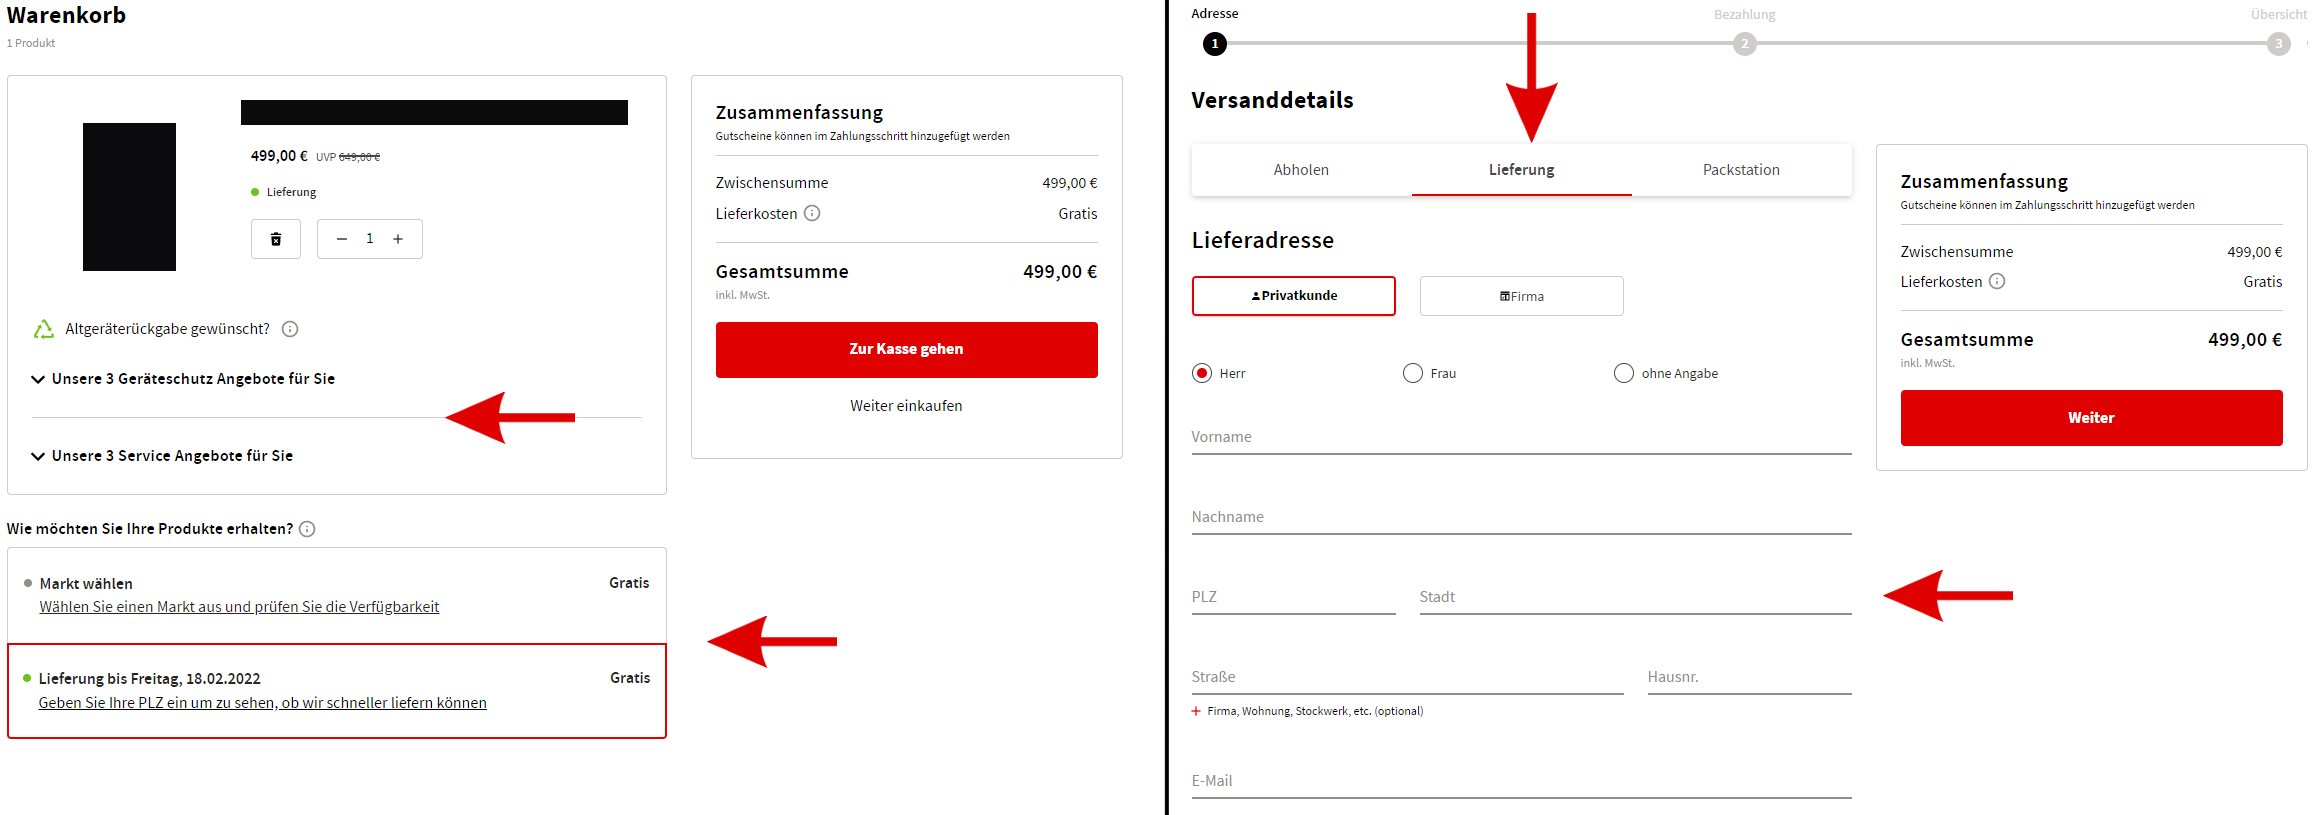
\includegraphics[width=\linewidth]{bilder/Checkout.png}
	\caption{Aktueller Checkout-Prozess des Onlineshops von MediaMarkt.de}
	\label{fig:Checkout-Process}
\end{figure}

Eine Neukalkulation findet statt sofern die Anzahl der Produkte im Warenkorb oder die Lieferkosten manipuliert werden. Ersteres kann außerhalb des Warenkorbs geschehen oder durch Hinzufügen von Services während der Anzeige des Baskets. Ebenfalls kann die Fulfillment-Methode und Lieferadresse angepasst werden, wodurch sich die Lieferkosten ändern können. Somit existieren einige Anwendungsfälle in denen eine Transaktion über beide Aggregate hinweg notwendig ist.

\textbf{Gibt es Invarianten zwischen den Warenkorb und den CalculationResult?}

Die Businessanforderung, dass das Berechnungsergebnis stets aktuell sein muss, wurde bereits gelockert. Verbleibend ist es zudem Notwendig aus rechtlichen Gründen, dass sich der Preis nach Initiierung des Bezahlvorgangs nicht ändert. Dieses Problem kann allerdings nicht auftreten, da der Warenkorb selbst nicht mehr manipuliert werden darf, somit bleibt der Gesamtpreis ebenfalls unberührt. Weitere Voraussetzungen existieren zum jetzigen Zeitpunkt nicht, jedoch müssen eventuelle zukünftige Anwendungsfälle berücksichtigt werden, ansonsten kann die Flexibilität der Anwendung gefährdet sein. 

Zur Veranschaulichung kann Auswirkungen einer neuen Regelung untersucht werden. Beispielsweise wird angenommen, dass der Gesamtpreis eines Warenkorbs nicht über 20.000€ liegen darf. In diesem Fall würde eine Anpassungen des Basket auch eine Neukalkulation benötigen, wodurch die Abtrennung des CalculationResults sinnfrei wird. Allerdings kann eine mildere Form dieser Richtlinie keine negativen Effekt besitzen, indem die Prüfung erst bei der Initiierung des Bezahlvorgangs ausgeführt wird, da zu diesem Zeitpunkt beide Aggregates immer synchron sind und keine Änderungen mehr erfahren können. Weitere erdenkbaren zukünftige Businessanforderungen sollten berücksichtigt werden, bevor ein Neudesign der Applikation durchgeführt wird.

Grundsätzlich scheint eine Abspaltung der Berechnungsergebnisse vom Warenkorb durchaus plausibel zu sein. Diese Vorgehensweise der Analyse kann analog auf verschiedene Anwendungsfälle durchgeführt werden, um weitere Teile des Baskets zu finden, welche separat agieren können. 

%TODO: Gleiche Überschrift oder nciht?
\subsection{Herausschneiden der Checkout-Daten aus dem Basket-Aggregate}

In dem Swimlane Diagramm \ref{fig:SL-Checkoutdata} wurde das Hinzufügen der Kundendaten, Bezahlungsmethode und Fulfillment beschrieben. Dieser Prozess ist ein Hinweise darauf, dass diese Daten eventuell aus dem Basket-Aggregat genommen werden können. Die Summe der Attribute wird als 'Checkout-Daten' betitelt und beinhalten Kundendaten, Fulfillment, Rechnungs- und Lieferadresse. Nachteilig ist jedoch, dass dadurch die Value Objects zu einer Entity zusammengefasst werden, da die Rolle des Aggregate Root nur durch Entities verfüllt werden darf. Ähnlich zum vorgehenden Unterkapitel ist eine Untersuchung der Implikationen eines solches Aggregationsschnittes notwendig.

Anpassungen an diesen Daten dürfen nur durchgeführt werden, wenn der Basket im Status 'open' ist. Dadurch muss bei jedem API-Aufruf zuvor der Zustand überprüft und der Warenkorb-Datenbankeintrag gesperrt werden. Aufgrund von möglichen Interleavings kann ansonsten die Initiierung des Bezahlvorgang auf invalide Checkout-Data stattfinden. Weiterhin wird durch das Setzten eines neuen Fulfillments die Neuberechnung des Warenkorbs angestoßen und bei Übergabe eines Payments muss der PaymentProcess aktualisiert werden.

Vorteilhaft an dieser Variante ist, dass der Basket leichtgewichtiger wird und geringere Datenmengen transportiert werden müssen. Zusätzlich bleiben die negativen Auswirkungen der getrennten Collections in der Datenbank gering, da die Anpassungen der Checkout-Daten nur selten in den User Stories vorkommt.

\section{Zusammenführung der vorgehenden Aggregationsschnitte}

Als Ergebnis aller Analysen dieses Kapitels kann ein neuer, zusammengefasster Aggregationsschnitt gebildet werden.  

%TODO: Warum nicht BaskeItems trennen
%TODO: Add Bewertung zu allen Aggregationsschnitte

\begin{figure}[htbp]
	\centering
	\includesvg[inkscapelatex=false, width=0.80\textwidth]{svg/VarD.svg}
	\caption{Aggregationsschnitt der Variante D}
	\label{fig:VarD}
\end{figure}


%TODO: Implementierung der Variante